\section{Results}\label{sec:results}
In this section we let the Q-learning algorithm act on the the state spaces described in section \ref{sec:bjMDP}. First, let $S_{hand}=\{  (s_{p1},\ldots,s_{p10},\Sigma_{d})\ s_{pi} \in \{1,2,\ldots, 21 \}, \Sigma_{d}\in \{1,2,\ldots, 10 \} \}$ and $S_{sum}=\{  (\Sigma_p, a_p, \Sigma_d )  \}$ denote the two state spaces. For abbreviation we may call these ``hand''- and ``sum''- environments or state spaces respectively. Also, we will simply call our Q-learning algorithm the ``algorithm''.

We will employ the algorithm on the two state spaces. In each simulation the values of the matrix $Q$ are initialized to zero. The constant $\eps$ is set (dynamically) according to the algorithm and theory described in Section \ref{sec:paramchoices}. The number of episodes is set to $10^7$ if not stated otherwise. 

In Figure \ref{fig:avg_return} we display the average return by episodes, of the algorithm for different number of decks. The x-axis is scaled to a proportion of the number of simulations performed. In the top left Figure of \ref{fig:avg_return}, denoted \ref{sfig:nd1}, we can see the performance of the Q-learning algorithm for 1 deck. Here, it becomes increasingly important to remember what cards that have been played. This is to be expected. When playing using one deck, there are only 4 of each card with the exception of all suites which are ten. Conditioned on the dealers outcome (where only one card is visible), the probability of seeing a arbitrary sequence of cards is relatively large for small deck sizes. However, as the deck size increases the information of what cards that are in the agents hand become redundant. This can be seen subsequently in Subfigures \ref{sfig:nd2}, \ref{sfig:nd8} and \ref{sfig:ndinf}. 

There is a specific shape to the left tail of the avg reward on the hand space seen in all figures of Figure \ref{fig:avg_return}. The behavior can be motivated by the cardinality of the hand space. In the first iterations, the algorithm visits a new state \textit{all the time}. It will take random actions almost always, just because of the cardinality. However, we can also note that the algorithm on the hand space learns faster in comparison to the algorithm on the sum in terms of average rewards. 
   
One can note that in all subfigures of \ref{fig:avg_return}, the algorithm seem to have some reward left to accumulate. It has not yet converged in neither state space. More simulations where not performed because of the lack of time and computational power. 

\begin{figure}[htp]
\begin{tabular}{cc}
\centering
 \begin{subfigure}[b]{0.48\textwidth}
  	 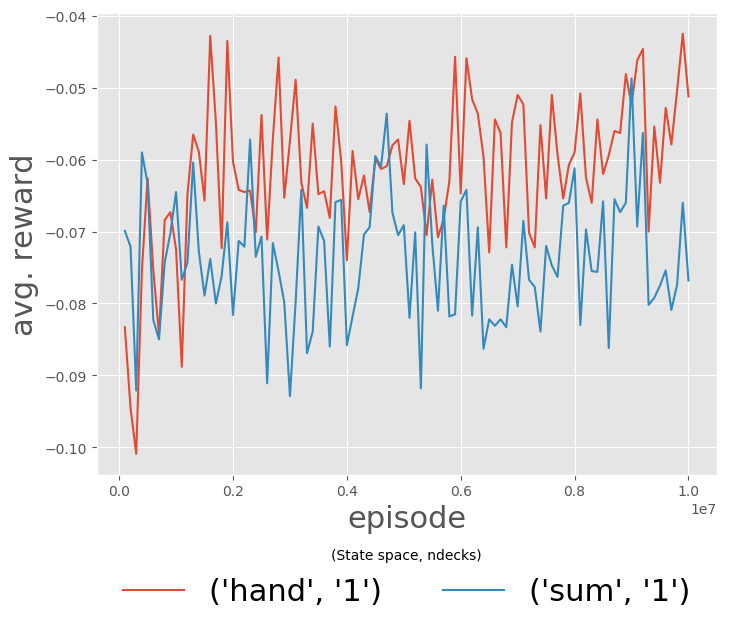
\includegraphics[width=\textwidth]{./figures/avgReturnEp_ndeck1.png}
   % .: 0x0 pixel, 0dpi, 0.00x0.00 cm, bb=
   \caption{Avg. return with 1 deck\label{sfig:nd1}}
 \end{subfigure}
 &
 \begin{subfigure}[b]{0.48\textwidth}
  	 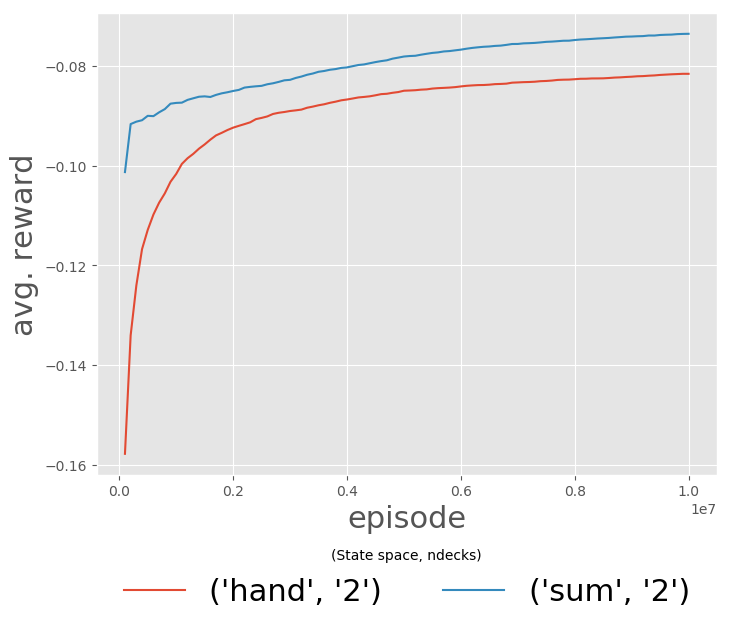
\includegraphics[width=\textwidth]{./figures/avgReturnEp_ndeck2.png}
   % .: 0x0 pixel, 0dpi, 0.00x0.00 cm, bb=
   \caption{Avg. return with 2 decks\label{sfig:nd2}}
 \end{subfigure}
 \\
 \begin{subfigure}[b]{0.48\textwidth}
  	 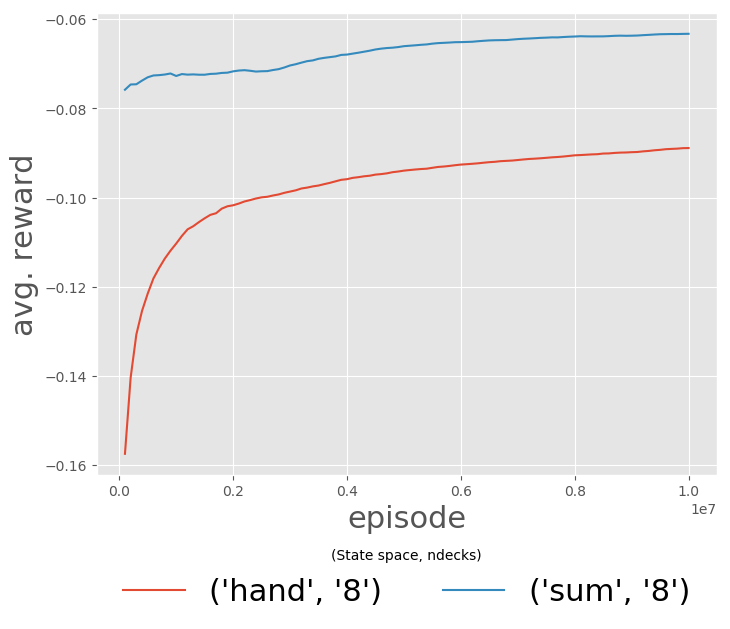
\includegraphics[width=\textwidth]{./figures/avgReturnEp_ndeck8.png}
   % .: 0x0 pixel, 0dpi, 0.00x0.00 cm, bb=
   \caption{Avg. return with 8 decks \label{sfig:nd8}}
 \end{subfigure}
 &
 \begin{subfigure}[b]{0.48\textwidth}
  	 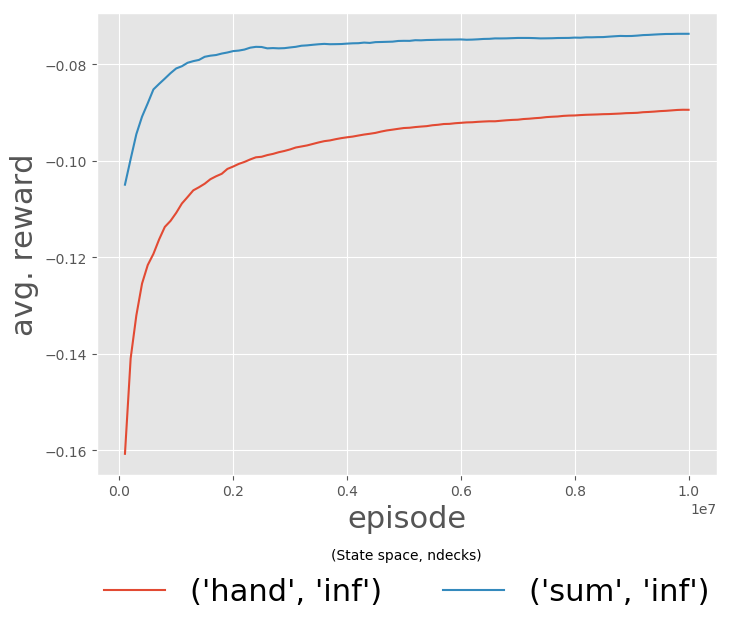
\includegraphics[width=\textwidth]{./figures/avgReturnEp_ndeckinf.png}
   % .: 0x0 pixel, 0dpi, 0.00x0.00 cm, bb=
   \caption{Avg. return with infinite decks \label{sfig:ndinf}}
 \end{subfigure}
\end{tabular}
\caption{The average return of the Q-learning algorithm for $1,2,8$ and $\infty$ number of decks. \label{fig:avg_return}}
\end{figure}

Since the cardinality of the hand space is much (!) larger than the sum's, the number of states the algorithm must explore will be larger. In Table \ref{tab:state_visited} we show the number of states the algorithm has explored together with the effective training time for the specific environment and the number of decks in play. We can clearly see that the number of explored states grows large for the hand state when the number of decks is increased. The number of states explored by the algorithm on the hand state space seem to converge to a level of $70 000$. As noted in section \ref{sec:stationaryMDP}, the number of effective states to be explored are not as grand as the actual state space. Hence, it is not surprising that the algorithm converge to level of states that are both necessary and valuable to explore. The algorithm fluctuates below 700 explored states for all deck sizes when learning on the sum space.

The training time for the algorithm on the hand space is large compared to the sum's. There is an indication that there is a $50\%$ increase in training time for the algorithm on the hand state compared to the sum. Note that the effective training time is simply the time it took to train this specific instance. All other measures of training time (which might be more accurate) are omitted because of the lack of computational power and time. 
\begin{table}[h!]
\centering
 \begin{tabular}{c|cc|cc}
  \# decks & $\#S_{hand}$ & $t_{hand}$ & $\#S_{sum}$ &  $t_{sum}$  \\
  \hline 
  $1$ & $7651$ & $1510.681$ & $641$ & $1003.765$ \\
  $2$ & $38266$ & $1565.314$ & $677$ & $1079.656$ \\
  $8$ & $70034$ & $1606.944$ & $695$ & $1079.626$ \\
  $\inf$ & $70307$ & $1636.044$ & $671$ & $1097.971$ 
 \end{tabular} 
 \caption{The number of explored states $\#S$ and the training time $t$ (seconds) for a given number of decks in play and its respective state space. The number of simulations was set to $10^7$.\label{tab:state_visited}}
\end{table}

Since estimates of Q-learning will converge to the true optimal value-action function we would like to visualize these said values. However, an obstacle in comparing the algorithm between the two spaces the cardinality of the hand poses a problem. The two state spaces do not align. Therefore, we will perform a (somewhat arbitrary) aggregation scheme. Each state of $S_{hand}$ will be transformed to a sum of the card values of that hand and if the ace was usable or not. We will take a simple average of the q-values when doing so. Post this aggregation scheme, the results from the algorithm on the hand space are now on the same form as the sum's. Then, we use our policy and take the maximum value of the two $q$-values corresponding to different action values of that state. In Figures \ref{sfig:3Dnd1} through \ref{sfig:3Dnd4} we have visualized the aggregated q-values for the hand state and the sum states, for different a deck size of size 1. The figures are divided into the case when the player holds a usable ace or not. Since the states where $\Sigma_d > 11$ are terminal we chose not to include them in this visualization.

From Figures  \ref{sfig:3Dnd1} through \ref{sfig:3Dnd4}, it is clear that holding a card sum of 21 indicates a large reward when using our policy. This is almost regardless of what the dealer is showing. This is satisfactory since it should be the best possible hand for an agent to hold.  The only exception is when the dealer draws an ace as its first card. As seen in Figure \ref{sfig:3Dnd2}, the value our policy when the dealer is showing an ace (first card) is relatively low. This is true through all states of the player sum. The same phenomena is seen in Figure \ref{sfig:3Dnd3} which, to some extent, eliminates the possibility of that this would be a result of the aggregation scheme. 

In general, when an ace is usable it cuts losses. This can be seen by comparing the pair of Figures \ref{sfig:3Dnd1} and \ref{sfig:3Dnd3} compared to Figures \ref{sfig:3Dnd2} and \ref{sfig:3Dnd4}. The amount of losses are generally less (less blue) in each state space for usable aces. This can be motivated by the flexibility a usable ace gives the player. By using the same pairs of Figures, it is also apparent that if the player has no usable ace then the value of the policy is higher for values close to 21. The slope of the ''hill'' is less when the player has no usable ace. 

\begin{center}
\begin{figure}[H]
  	 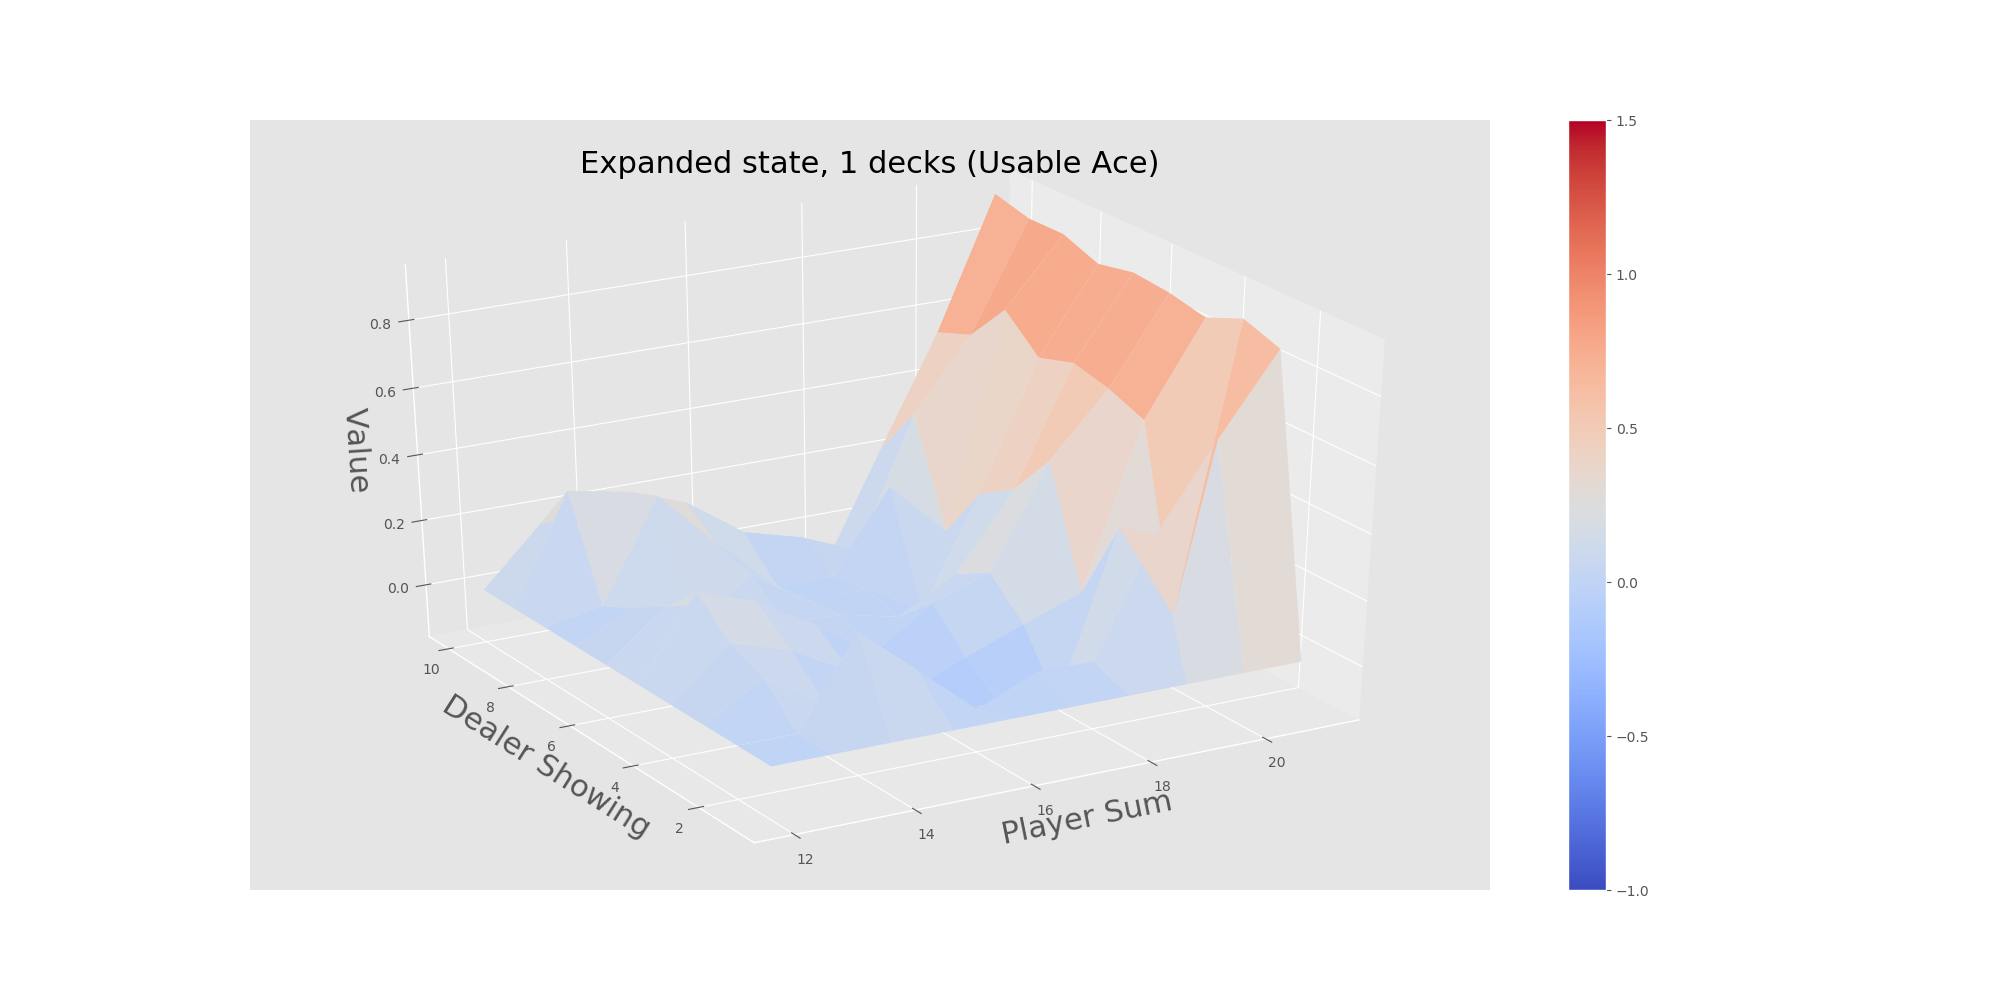
\includegraphics[width=1.2\textwidth]{./figures/ace_3D_exp_1_decks.png}
   % .: 0x0 pixel, 0dpi, 0.00x0.00 cm, bb=
   \caption{Aggregated q-values when the player has an usable ace.\label{sfig:3Dnd1}}
\end{figure}
 \begin{figure}[H]%{\textwidth}
  	 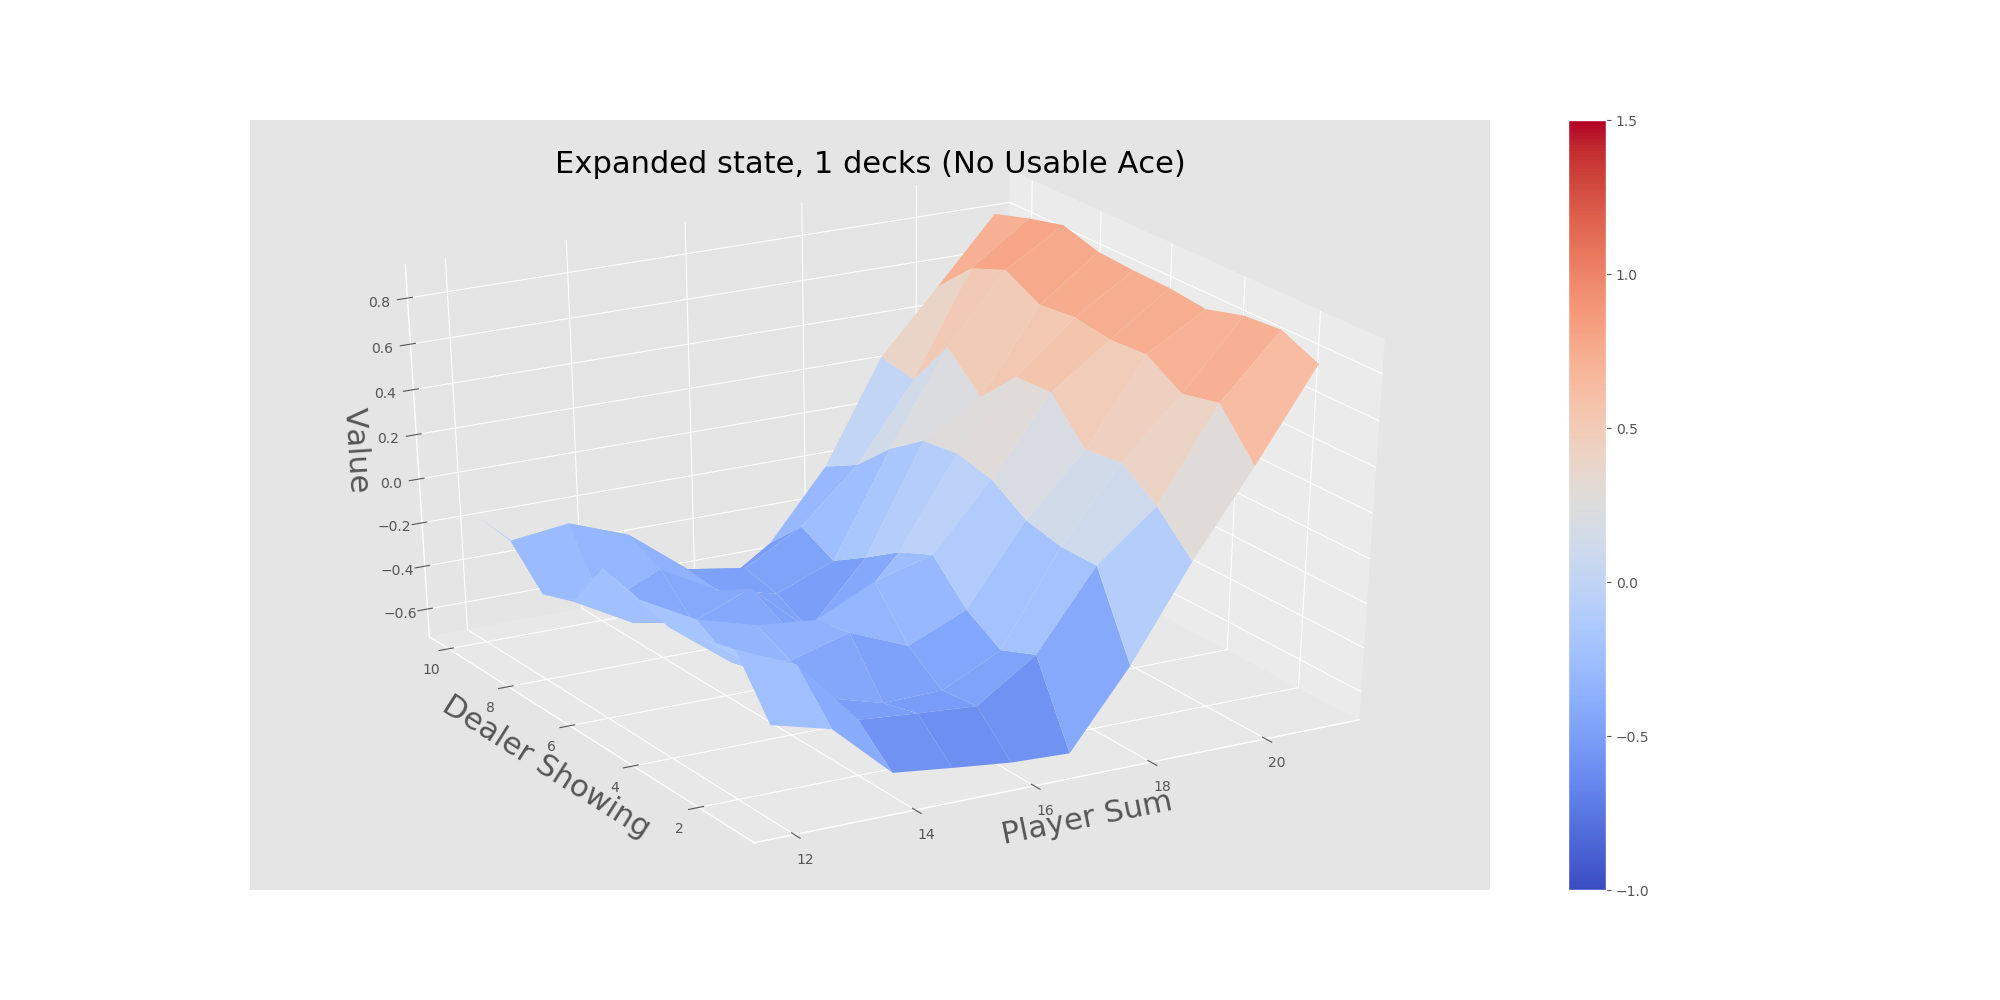
\includegraphics[width=1.2\textwidth]{./figures/noace_3D_exp_1_decks.png}
   % .: 0x0 pixel, 0dpi, 0.00x0.00 cm, bb=
   \caption{Aggregated q-values when the player has no usable ace.\label{sfig:3Dnd2}}
 \end{figure}
 \begin{figure}[H]%{\textwidth}
  	 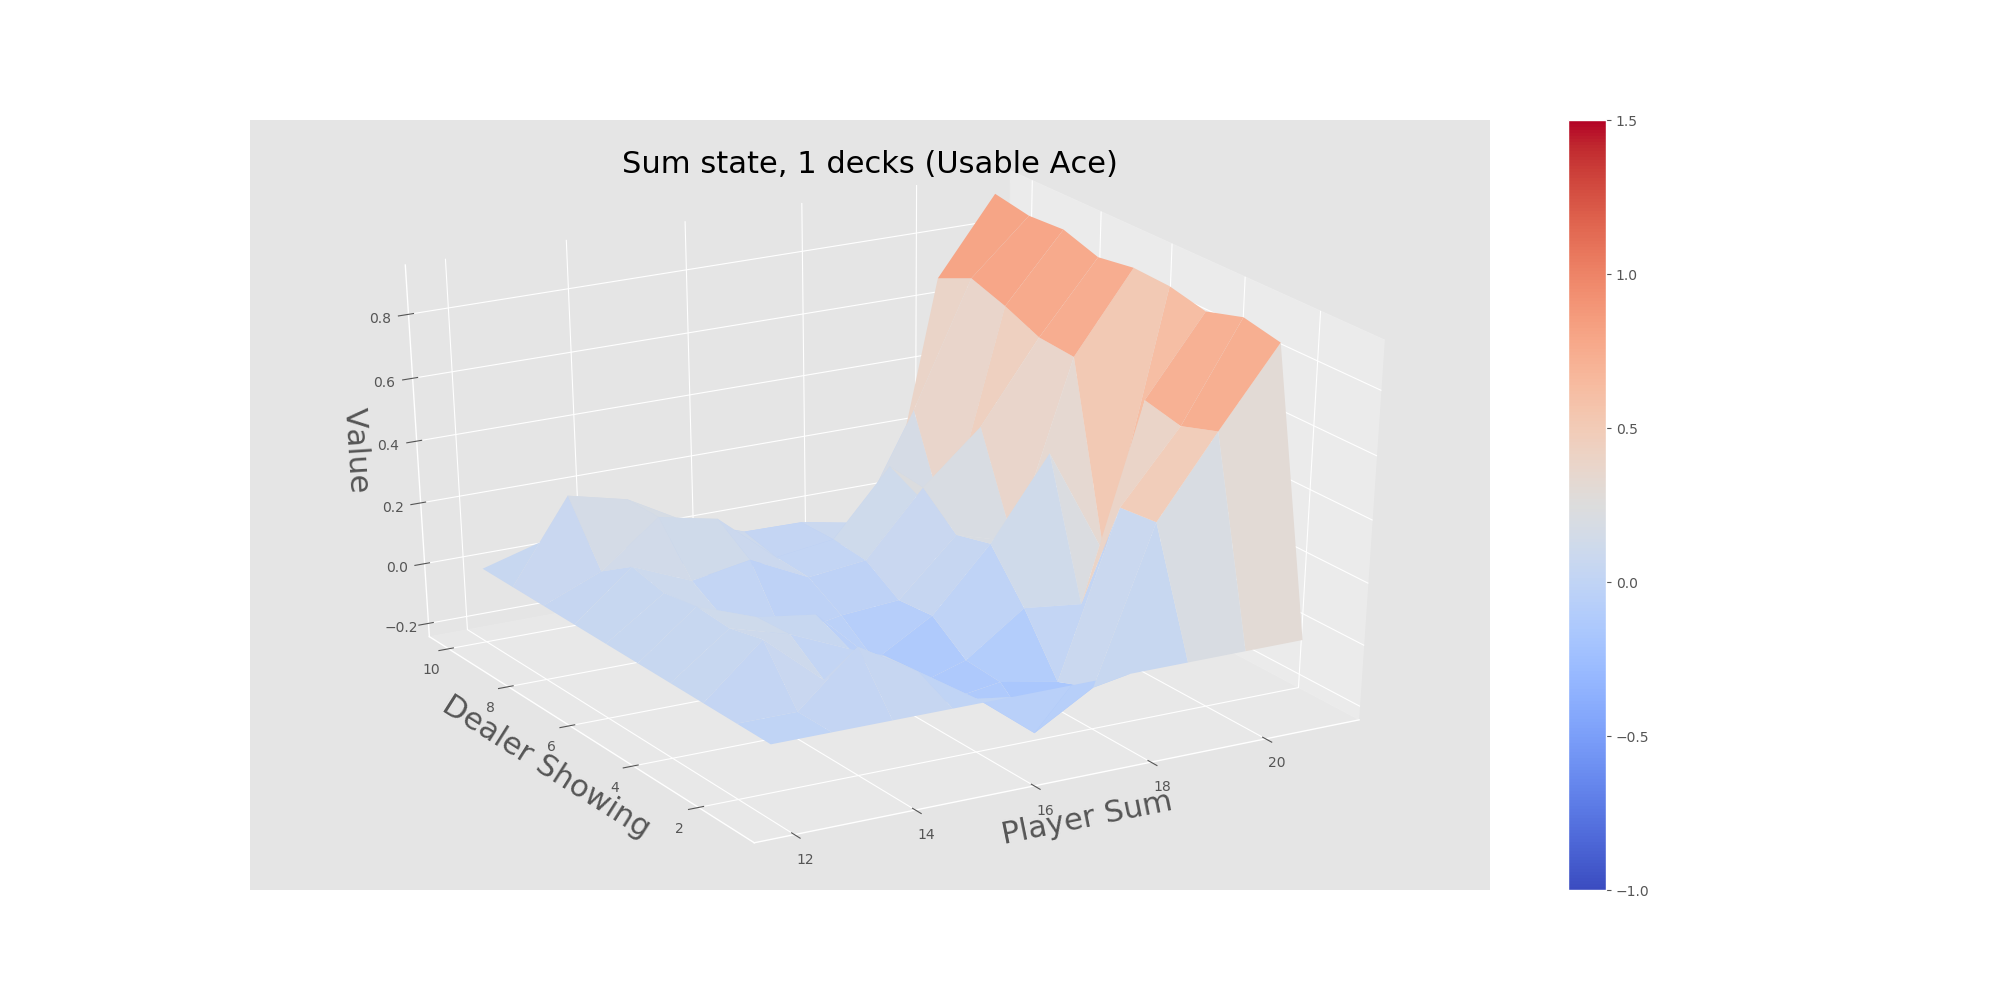
\includegraphics[width=1.2\textwidth]{./figures/ace_3D_sum_1_decks.png}
   % .: 0x0 pixel, 0dpi, 0.00x0.00 cm, bb=
   \caption{Q-values when the player has an usable ace. \label{sfig:3Dnd3}}
 \end{figure}
 \begin{figure}[H]%{\textwidth}
  	 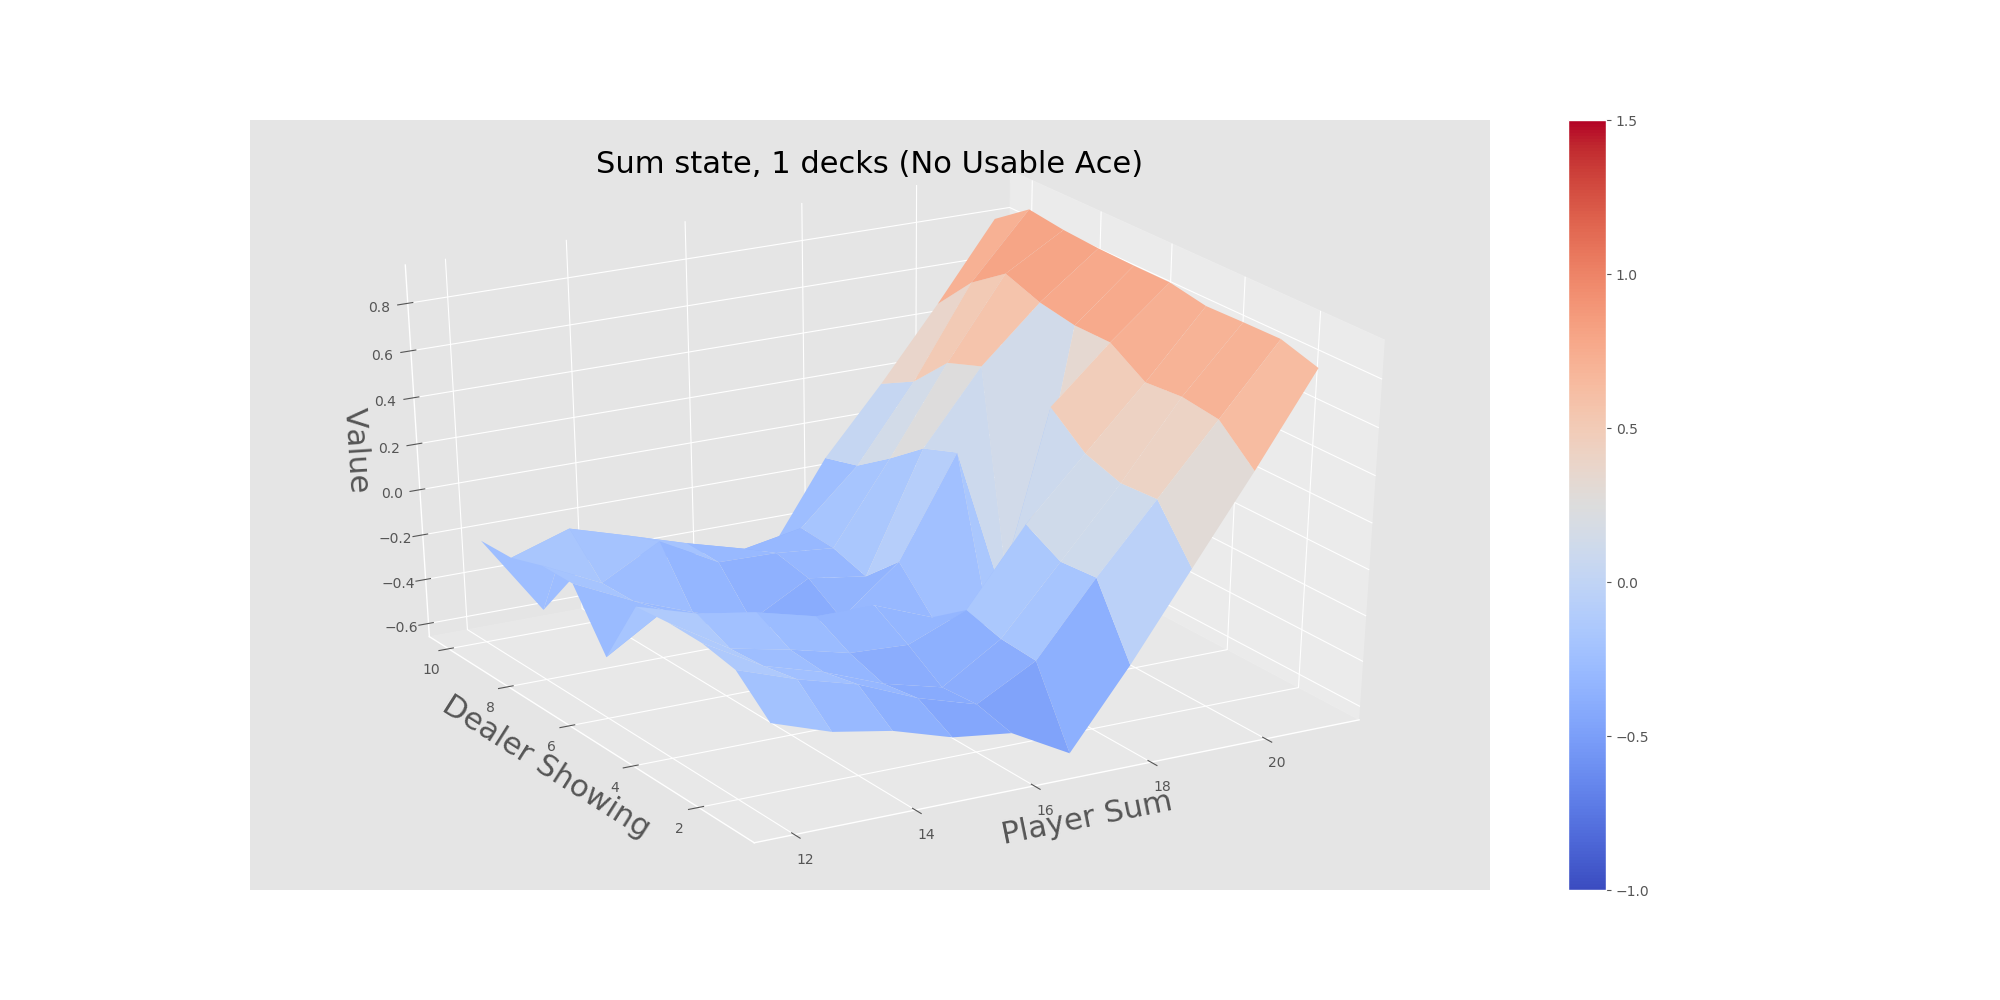
\includegraphics[width=1.2\textwidth]{./figures/noace_3D_sum_1_decks.png}
   % .: 0x0 pixel, 0dpi, 0.00x0.00 cm, bb=
   \caption{Q-values when the player has no usable ace. \label{sfig:3Dnd4}}
 \end{figure}
\end{center}
